% Created 2012-10-18 Thu 13:03
\documentclass[a4paper]{article}
\usepackage[utf8]{inputenc}
\usepackage{hyperref}
\usepackage{graphicx}
\usepackage{longtable}
\usepackage{float}
\usepackage{pdfpages}
\providecommand{\alert}[1]{\textbf{#1}}

\title{ADA-NCEPH Data Access Procedure}
\author{Ivan Hanigan and Steven McEachern}
\date{\today}
\hypersetup{
  pdfkeywords={},
  pdfsubject={},
  pdfcreator={Emacs Org-mode version 7.8.11}}

\begin{document}

\maketitle

% Org-mode is exporting headings to 3 levels.
\tableofcontents

\clearpage
\section{TODOLIST}
\label{sec-1}
\subsection{\textbf{TODO} Ivan change registry to ANU-DB}
\label{sec-1-1}
\subsection{\textbf{TODO} Ivan send to steve by noon Fri.}
\label{sec-1-2}
\subsection{\textbf{TODO} Steve review and comment}
\label{sec-1-3}
\subsection{\textbf{TODO} Ivan revise and send to BDM by Wed-ish}
\label{sec-1-4}
\section{Introduction}
\label{sec-2}

The aim of this document is to describe the procedure for accessing restricted health data through the proposed ANU Secure Data Hub, administered by the ADA and NCEPH.

The following descibes roles and processes for:
\begin{itemize}
\item Users
\item User Admins
\item Data Admins
\end{itemize}

The User and Data information is stored in a Database at ANU referred to as ANU-DB.
\section{Getting Access}
\label{sec-3}

  
\subsection{Flow Chart of Steps to Get Access}
\label{sec-3-1}

\begin{figure}[!h]
\centering
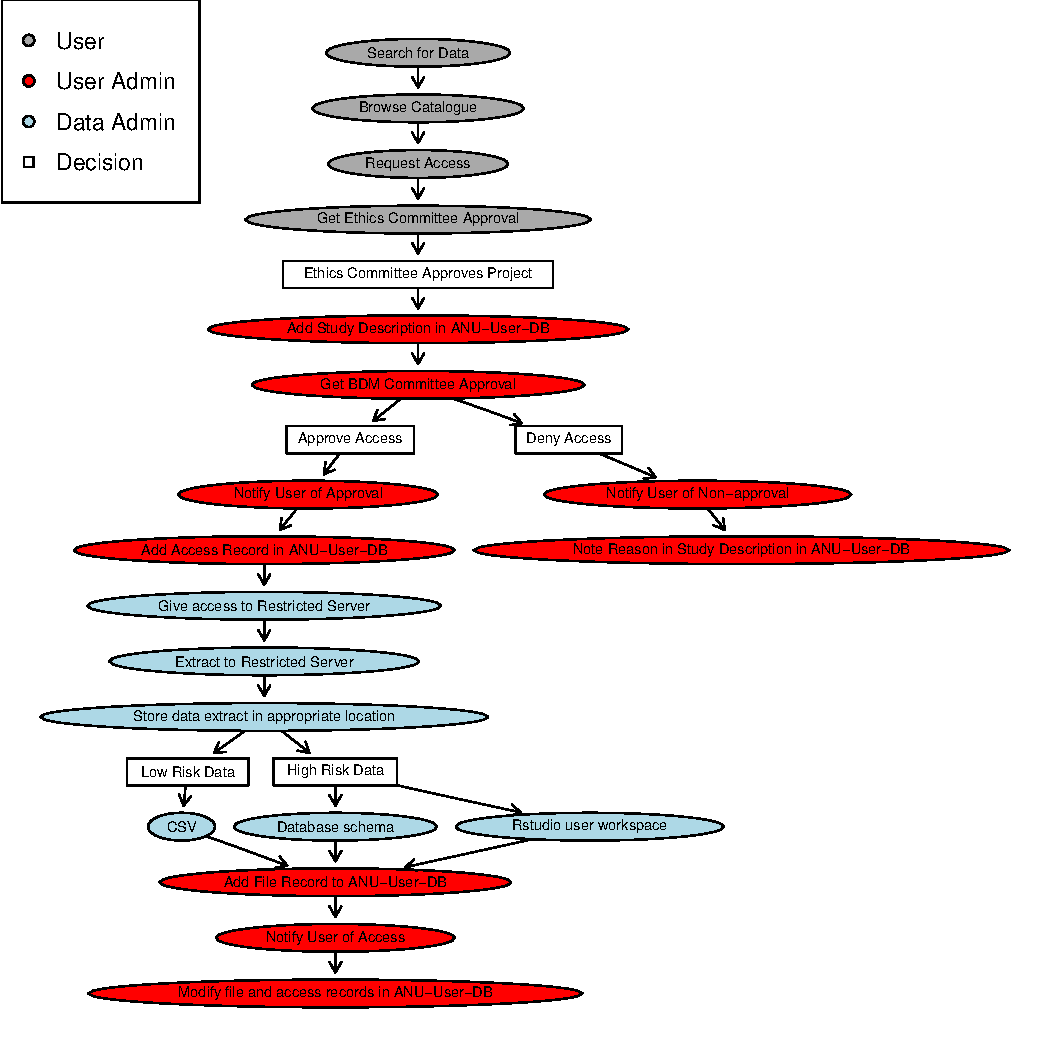
\includegraphics[width=\textwidth]{DataAccessFlowDiagram-GettingAccess.pdf}
\caption{DataAccessFlowDiagram-GettingAccess}
\label{fig:DataAccessFlowDiagram-GettingAccess}
\end{figure}
\clearpage
\section{Managing Access}
\label{sec-4}
\subsection{Query Lists of Projects and Users}
\label{sec-4-1}

This is biannual or annual.
\subsection{Flow Chart of Steps to Manage Access}
\label{sec-4-2}


\begin{figure}[!h]
\centering
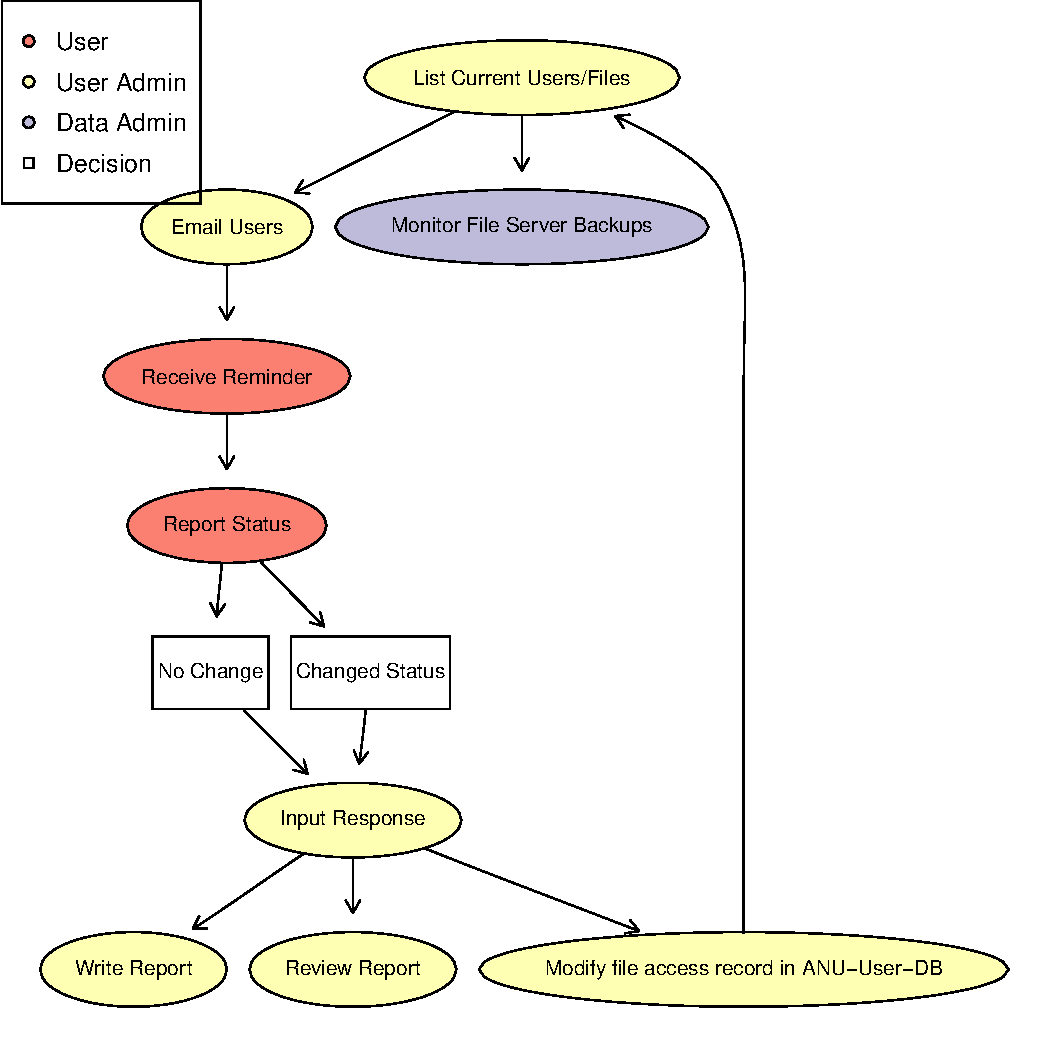
\includegraphics[width=\textwidth]{DataAccessFlowDiagram-ManagingAccess.pdf}
\caption{DataAccessFlowDiagram-ManagingAccess}
\label{fig:DataAccessFlowDiagram-ManagingAccess}
\end{figure}
\clearpage
\section{Ending Access}
\label{sec-5}
\subsection{Flow Chart for Ending Access}
\label{sec-5-1}
\subsection{Flow Chart of Steps to Manage Access}
\label{sec-5-2}


\begin{figure}[!h]
\centering
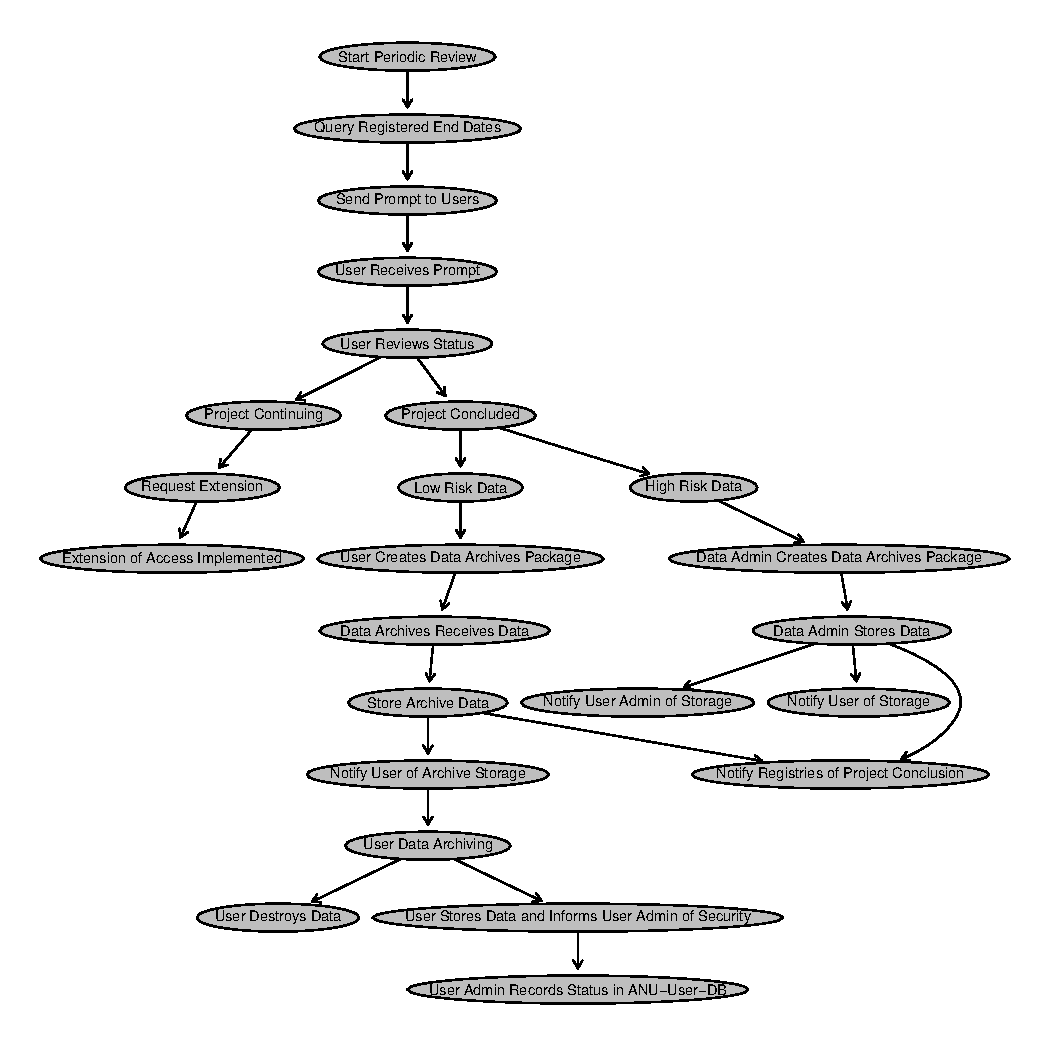
\includegraphics[width=\textwidth]{DataAccessFlowDiagram-EndAccess.pdf}
\caption{DataAccessFlowDiagram-EndAccess}
\label{fig:DataAccessFlowDiagram-EndAccess}
\end{figure}
\clearpage
\section{Visualise the Data Access Process}
\label{sec-6}

\end{document}